%% LyX 2.3.7 created this file.  For more info, see http://www.lyx.org/.
%% Do not edit unless you really know what you are doing.
\documentclass[english]{book}
\usepackage[latin9]{inputenc}
\usepackage[a4paper]{geometry}
\geometry{verbose,tmargin=2cm,bmargin=2cm,lmargin=1in,rmargin=1.5cm}
\usepackage{fancybox}
\usepackage{calc}
\usepackage{textcomp}
\usepackage{amsmath}
\usepackage{makeidx}
\makeindex
\usepackage{graphicx}

\makeatletter
%%%%%%%%%%%%%%%%%%%%%%%%%%%%%% Textclass specific LaTeX commands.
\@ifundefined{lettrine}{\usepackage{lettrine}}{}

\makeatother

\usepackage{babel}
\begin{document}
\title{A Complete Course in Physics ( Graphs ) - Extended First Edition}
\author{Rajat Kalia and Pooja Duggal}
\date{March 09, 2017}
\maketitle

\chapter*{Preface}

The First Edition was a collection of tough problems but the file
was small , only being 12 pages not meeting the Amazon crieteria of
minimum 24 pages for paperback printing. Moreover, the toughness of
problems required that answers be provided Intext. 

Graphs is a very catchy topic for +1/+2 level and Competitive Exams,
it is apparent that books in this particular topic would be written
and available soon in the near future.

\chapter*{Acknowledgements}

I first of all thank my son Manas Kalia for the love and support.

Today, he is writing an essay on ``Myself'' for all of us

\doublebox{\begin{minipage}[t]{0.7\columnwidth}%
1 My name is Manas.

2 I am six years old.

3 I study in KGF.

4 I like to play ludo.

5 I love my family.%
\end{minipage}}

I would also like to show few of his designs, he has made while playing
on computer.

\doublebox{\begin{minipage}[t]{0.7\columnwidth}%
\includegraphics[scale=0.5]{\string"Images/CC/P-Graphs/1e-1.1e/ManasImgsSlctd/BaloonSeller2 001\string".jpg}%
\end{minipage}}

\doublebox{\begin{minipage}[t]{0.7\columnwidth}%
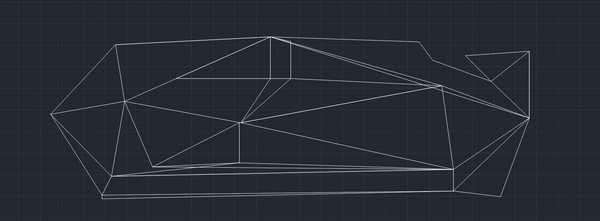
\includegraphics[scale=0.5]{Images/CC/P-Graphs/1e-1.1e/ManasImgsSlctd/Drawing4}%
\end{minipage}}

\doublebox{\begin{minipage}[t]{0.7\columnwidth}%
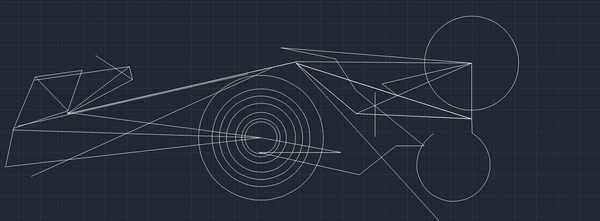
\includegraphics[scale=0.5]{Images/CC/P-Graphs/1e-1.1e/ManasImgsSlctd/Drawing6}%
\end{minipage}}

\doublebox{\begin{minipage}[t]{0.7\columnwidth}%
\includegraphics[scale=0.5]{\string"Images/CC/P-Graphs/1e-1.1e/ManasImgsSlctd/Holi 001\string".jpg}%
\end{minipage}}

\doublebox{\begin{minipage}[t]{0.7\columnwidth}%
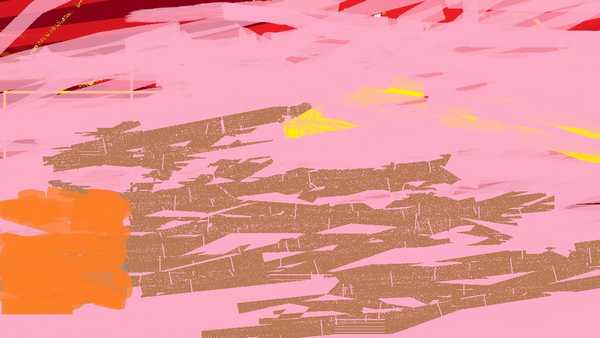
\includegraphics[scale=0.5]{Images/CC/P-Graphs/1e-1.1e/ManasImgsSlctd/Untitled7}%
\end{minipage}}

\doublebox{\begin{minipage}[t]{0.7\columnwidth}%
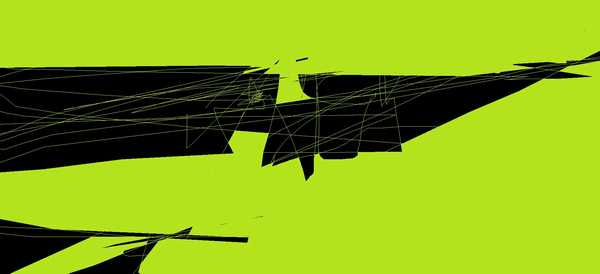
\includegraphics[scale=0.5]{Images/CC/P-Graphs/1e-1.1e/ManasImgsSlctd/Untitled19}%
\end{minipage}}

\tableofcontents{}

\chapter{Concepts of Graphs}

\section{The Equations of motion and the origin of Graph Handling}

\subsection{\index{The First Equation}The First Equation}

The Equation $v=\dfrac{dx}{dt}$ in linear motion implies
\begin{quote}
i) The \textbf{Slope} of \textbf{Position-Time Graph} is \textbf{Instantaneous
Velocity.}

ii) The \textbf{Area} under the \textbf{Velocity-Time Graph} is \textbf{Change
in Position}.

\{ The second one requires the manipulation , $dx=vdt$ i.e. $\int dx=\int vdt$
\} 
\end{quote}
The equations can be further manipulated to obtain the Speed Time
Graph , where 
\begin{quotation}
speed = rate of change of distance wrt time 
\end{quotation}
Few of the following examples illustrate this concept: 
\begin{description}
\item [{Example:}] On a displacement-time graph, two straight lines make
angles of 30� and 60� with the time-axis. The ratio of the velocities
represented by them is 
\end{description}
\begin{quote}
a) $1:\sqrt{3}$

b) 1:3

c) $\sqrt{3}:1$

d) 3:1

\{ Hint: The velocity in a displacement-time is given by the slope
of the curve. Slope = tan(gent) of angle of inclination of s-t graph.
This gives the respective ratios tan 30$^{o}$ / tan 60$^{o}$ 

Answer: b) is the correct answer. \}
\end{quote}
\begin{description}
\item [{Example:}] A body is moving in a straight line as shown in velocity-time
graph. The displacement and distance travelled by body in 8 second
are respectively:
\end{description}
\doublebox{\begin{minipage}[t]{0.7\columnwidth}%
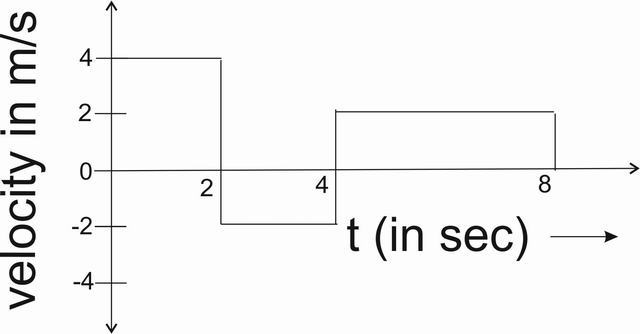
\includegraphics[scale=0.5]{Images/CC/P-Graphs/1e-1.1e/ImagesReduced/Q2-firstequation}%
\end{minipage}}
\begin{quote}
a) 12 m, 20 m

b) 20 m, 12 m

c) 12 m, 12 m

d) 20 m, 20 m

\{ Hint: The displacement in a velocity-time graph is given by the
area under the graph with proper signs. From 0s - to 2s , the area
is 8m . From 2s - to 4s , the area is -4m . From 4s - to 8s , the
area is 8m. Adding these 3 values , we get 8m + (-4m) + 8m = 12m.
\} The distance in a v-t graph is given by the absolute area under
the graph. So, taking the absolute values of individual area divisions,
we get 8m + 4m + 8m =20m

Answer: a) is the correct answer. \}
\end{quote}
\begin{description}
\item [{Example:}] The graph shows position as a function of time for two
trains running on parallel tracks. Which statement is true?
\end{description}
\doublebox{\begin{minipage}[t]{0.7\columnwidth}%
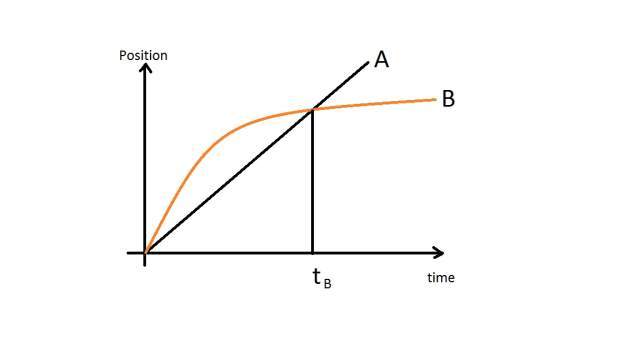
\includegraphics[scale=0.75]{Images/CC/P-Graphs/Common/Reduced/ClassicalApproach/Paralleltracktrains}%
\end{minipage}}
\begin{quote}
a) At time t$_{B}$ both trains have the same velocity.

b) Both trains have the same velocity at some time after t$_{B}$
.

c) Both trains have the same velocity at some time before t$_{B}$
.

d) Somewhere on the graph, both trains have the same acceleration.

\{ Hint: Depending on the question requirements, we'll have to check
all the assertions one by one.

a) In a position time graph, the slope gives velocity. It can be clearly
seen that Graph B has a much lower slope than Graph A at time $t_{B}$.
So, the assertion is wrong.

b,c) By drawing a line parallel to the line A which is a tangent to
Graph B , it can be seen where the two graphs have same slope. It
is clear that the graphs have same slope between 0 and $t_{B}$ as
noted from the figure. So, assertion b is wrong while c is correct.

\doublebox{\begin{minipage}[t]{0.7\columnwidth}%
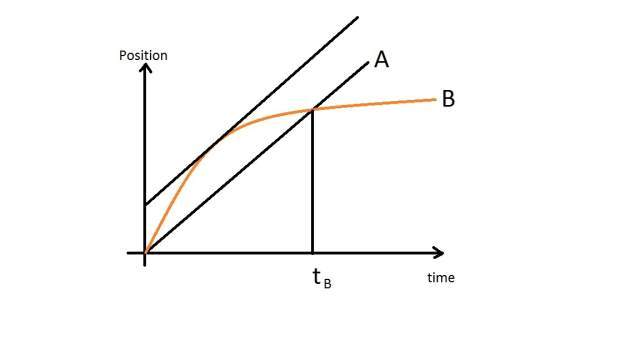
\includegraphics[scale=0.75]{Images/CC/P-Graphs/Common/Reduced/ClassicalApproach/Paralleltracktrainssolution}%
\end{minipage}}

d) As the Graph A has a constant slope, so the acceleration of body
A is zero. Whereas Graph B is constantly turning, so the slope can
be assumed to be non-zero throughout. According to some revelations,
however it is noted that the figure is not clear enough to show whether
Graph B is straight after $t_{B}$ or bending. In case it is assumed
to be straight, then after $t_{B}$ both trains will have same (zero)
acceleration. Also at start both have large (infinite) accelration,
in which case the ratio of the two large ( infinite ) values may be
calculated if initial conditions are mentioned and is required.

At our level we would assume this assertion to be wrong, however making
a note that the image should have been more clearly presented.

Answer: c) is the correct assertion. \}
\end{quote}
\begin{description}
\item [{Example:}] The velocity-time graph of a particle in linear motion
is as shown. Both v and t are in SI units. The displacement of the
particle is
\end{description}
\doublebox{\begin{minipage}[t]{0.7\columnwidth}%
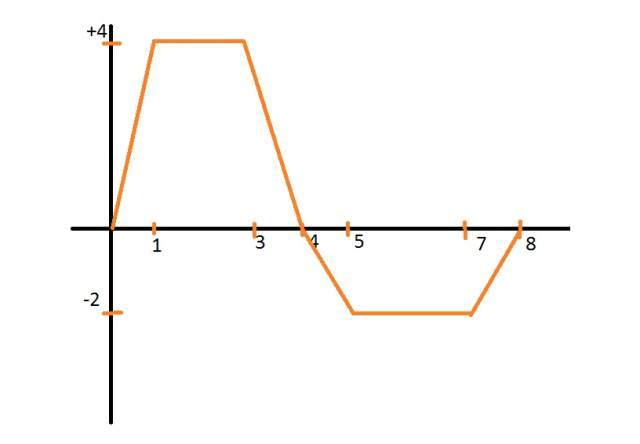
\includegraphics[scale=0.75]{Images/CC/P-Graphs/Common/Reduced/ClassicalApproach/displacementfromvtgraphproblem}%
\end{minipage}}
\begin{quote}
a) 6 m

b) 8 m

c) 16 m

d) 18 m

\{ Hint : For displacement calculations, between 0 - to 4 , area of
the positive trapesium = $\dfrac{1}{2}\times\left(2+4\right)\times4$
= 12

between 4 - to 8, area of negative trapesium =$\dfrac{1}{2}\times(2+4)\times(-2)$
= -6.

So , the answer is +6

So , a is the correct option.\}
\end{quote}

\subsection{\index{The Second Equation}The Second Equation}

Proceeding similar to above, the equation $a=\dfrac{dv}{dt}$ implies
\begin{quote}
i) The \textbf{Slope} of \textbf{Velocity-Time Graph} is \textbf{Instantaneous
Acceleration}.

ii) The\textbf{ Area} under \textbf{Acceleration-Time Graph} is \textbf{Change
in Velocity}.

\{ The second one requires the manipulation , $dv=adt$ i.e. $\int dv=\int adt$
\} 
\end{quote}
A few of the following examples illustrate it.
\begin{description}
\item [{Example:}] A car starts from rest acquires a velocity v with uniform
acceleration $2ms^{-2}$ then it comes to stop with uniform retardation
$4ms^{-2}$ . If the total time for which it remains in motion is
3 sec, the total distance travelled is:
\end{description}
\begin{quote}
a) 2 m

b) 3 m

c) 4 m

d) 6 m 

\{Hint: For solving this problem, we draw the graph of the problem, 

\doublebox{\begin{minipage}[t]{0.7\columnwidth}%
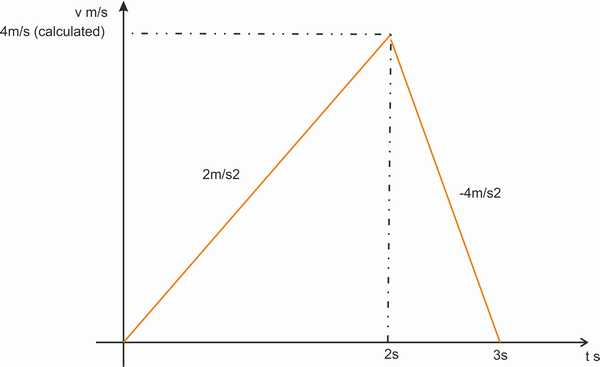
\includegraphics[scale=0.5]{Images/CC/P-Graphs/1e-1.1e/ImagesReduced/Q1-secondequation-Answers}%
\end{minipage}} 

Accordning to graph, let the time when it reaches maximum velocity
be T, and the maximum velocity be V. 

$\Rightarrow$V = 2XT and also V = 4X(3-T)

Equating the equations,

2T = 12-4T = V

$\Rightarrow$6T = 12

$\Rightarrow$T = 2

$\Rightarrow$ V = 2T = 4

Calculating the area under the graph using the calculated parameters,
Area = 1/2 X 4 X 3 = 6m

So , area under the graph is 6m = displacement . Also, as all the
area is on the positive side, so distance = 6m. 

\}
\end{quote}
\begin{description}
\item [{Example:}] A particle starts from rest. Its acceleration (a) vs
time (t) is as shown in the Figure. The maximum speed of the particle
will be
\item [{%
\doublebox{\begin{minipage}[t]{0.7\columnwidth}%
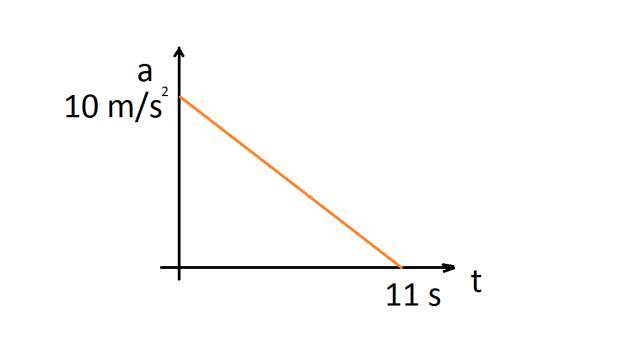
\includegraphics[scale=0.75]{Images/CC/P-Graphs/Common/Reduced/ClassicalApproach/accelerationvstime}%
\end{minipage}}}]~
\end{description}
\begin{quote}
a) 110 m/s

b) 55 m/s

c) 550 m/s

d) 660 m/s

\{ Hint : Writing the equation of the graph , we get $\dfrac{a}{10}+\dfrac{t}{11}=1$

$\Rightarrow$$a=\dfrac{10}{11}(11-t)$

Integrating, ( we will assume initial velocity to be zero as the body
starts from rest. )

$v=\dfrac{10}{11}(11t-\dfrac{1}{2}t^{2})$

Substituting $t=11s$

$v_{11s}=55m/s$

Answer: b) is the correct answer \}
\end{quote}
\begin{description}
\item [{Example:}] Acceleration-time graph of a particle moving in a straight
line is shown in Figure. The velocity of particle at time t = 0 is
2 m/s. Velocity at the end of fourth second is
\item [{%
\doublebox{\begin{minipage}[t]{0.7\columnwidth}%
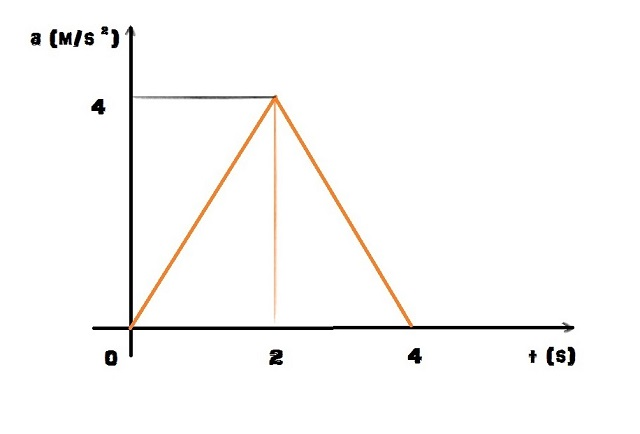
\includegraphics[scale=0.72]{Images/CC/P-Graphs/Common/Original/ClassicalApproach/acc-t-graph-3}%
\end{minipage}}}]~
\end{description}
\begin{quote}
a) 8 m/s

b) 10 m/s

c) 12 m/s

d) 14 m/s

\{ Hint: Area under the acceleration-time graph is change in velocity.
Area of the triangle is Half ( into ) base ( into ) altitude = 8m/s.
Adding the initial value of 2m/s , we get 2 + 8 = 10m/s. 

Answer: b) is the correct answer \}
\end{quote}
\begin{description}
\item [{Example:}] Each of the three graphs represents acceleration vs
time for an object that already has a positive velocity at time $t_{1}$
. Which graph/graphs show an object whose speed is increasing for
the entire time interva1 between $t_{1}$ and $t_{2}$ ?
\item [{%
\doublebox{\begin{minipage}[t]{0.7\columnwidth}%
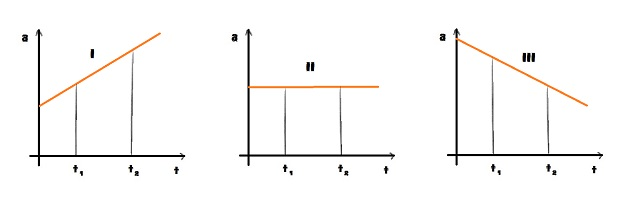
\includegraphics[scale=0.72]{Images/CC/P-Graphs/Common/Original/ClassicalApproach/ncertproblem}%
\end{minipage}}}]~
\end{description}
\begin{quote}
a) Graph I only

b) Graphs I and II

c) Graphs I and III

d) Graphs I, II and III

\{Hint: Area under the acceleration time graphs give change in velocity.
In all the three figures, the area under the graphs are +ve, hence
velocity is increasing in all cases. As the initial velocity is +ve
, in all three cases the velocity remains throughout positive. So
, the speed is also increasing in all cases.\}
\end{quote}
\begin{description}
\item [{Example:}] A body starts from rest and moves along a straight line
with constant acceleration. The variation of speed v with distance
s is given by the graph
\item [{%
\doublebox{\begin{minipage}[t]{0.7\columnwidth}%
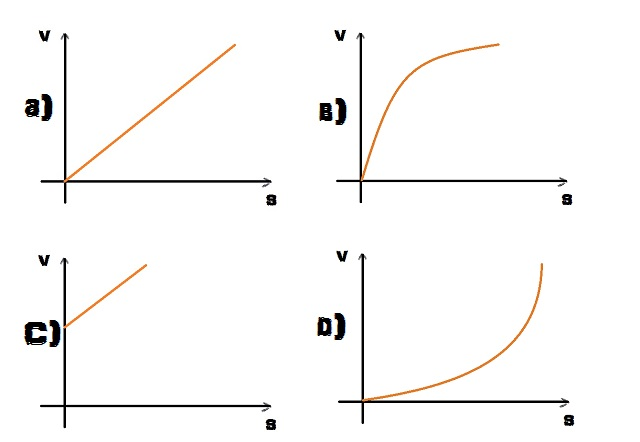
\includegraphics[scale=0.72]{Images/CC/P-Graphs/Common/Original/ClassicalApproach/Untitled2}%
\end{minipage}}}]~
\end{description}
\begin{quote}
\{ Hint: The problem given has $v_{o}$= 0 

Now acceleration = constant ( lets say k ) = $\dfrac{dv}{dt}$

$\Rightarrow$$k=v\dfrac{dv}{ds}$

$\Rightarrow$$\int_{0}^{v}vdv=\int_{0}^{s}kds$

$\Rightarrow$$v=\sqrt{2ks}$

The graph is proportional to square root function

Hence , b (as it is the only graph with such a property )

Answer : b) is the correct graph \}
\end{quote}

\subsection{\index{The Acceleration-Position Graph Variate}The Acceleration-Position
Graph Variate}
\begin{quote}
This kind of graph requires the manipulation of the Equation $a=\dfrac{dv}{dt}$
as follows

$a=\dfrac{dv}{dx}.\dfrac{dx}{dt}$

$\Rightarrow$$a=\dfrac{dv}{dx}.v$

$\Rightarrow$ $adx=vdv$ and integration can be performed to further
solve it.
\end{quote}
\begin{description}
\item [{Example:}] A body, initially at rest, starts moving along x-axis
in such a way that its acceleration vs displacement plot is as shown
in the Figure. The maximum velocity of the particle is
\item [{%
\doublebox{\begin{minipage}[t]{0.7\columnwidth}%
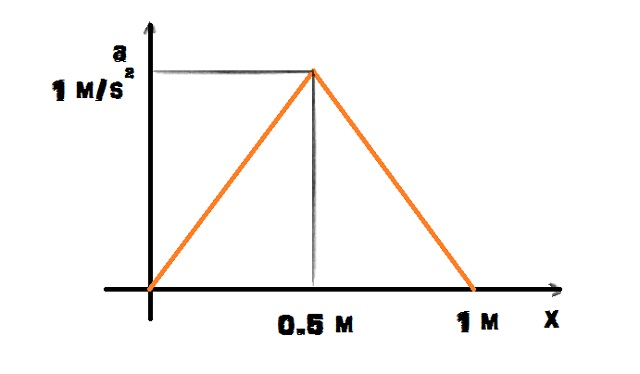
\includegraphics[scale=0.72]{Images/CC/P-Graphs/Common/Original/ClassicalApproach/accelerationposition1}%
\end{minipage}}}]~
\end{description}
\begin{quote}
a) 1 m/s

b) 6 m/s

c) 2 m/s

d) None of these

\{ Hint : The area under the a-x graph gives change in $\dfrac{v^{2}}{2}$
as can be evaluated by Integration method. The area of triange is
(0.5) X (1) X (1) = 0.5

$\Rightarrow$v = 1m/s . Initial position is given to be 0 in the
graph. Hence, we take only the positive sign.

Answer : a) is the correct answer. \}
\end{quote}
\begin{description}
\item [{Example}] : A particle initially at rest, it is subjected to a
non-uniform acceleration a, as shown in the gure. The maximum speed
attained by the particle is
\item [{%
\doublebox{\begin{minipage}[t]{0.7\columnwidth}%
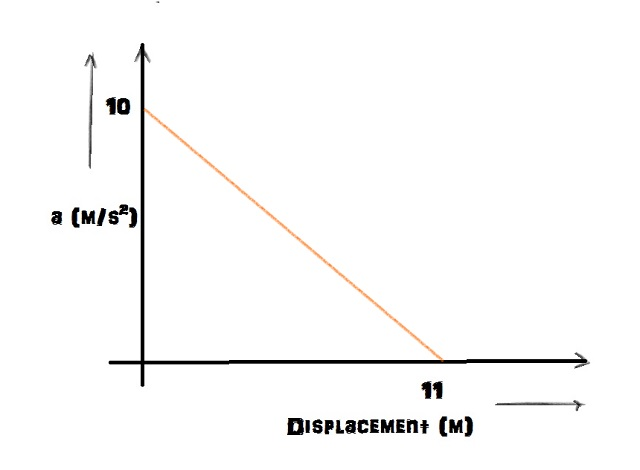
\includegraphics[scale=0.72]{Images/CC/P-Graphs/Common/Original/ClassicalApproach/acclnvsdisplacement}%
\end{minipage}}}]~
\end{description}
\begin{quote}
a) 605 m/s

b) 110 m/s

c) 55 m/s 

d) 110 m/s

\{ Hint: The area under the a-t graph is half the change in $v^{2}$.
Area under the graph is 55. So $v_{max}=\sqrt{110}m/s$ . Hence none
of the answers is correct \}
\end{quote}

\section{\index{Other Types of Graphs}Other Types of Graphs}

\subsection{\index{Sign of Acceleration from Position-Time Graph}Sign of Acceleration
from Position-Time Graph}
\begin{quote}
The sign of Acceleration can be determined from the Position-Time
Graph. The methodology involves of looking at the Concavity of the
Graph

i) If the graph is Concave-Up, the Acceleration is Positive.

ii) If the graph is Concave-Down, the Acceleration is Negative.

iii) If the graph is a straight line, the Acceleration is ZERO. \{
Irrespective of any other factor , such as the slope or direction
of line\} 
\end{quote}
\begin{description}
\item [{Example:}] The graph given below is a plot of distance vs time.
For which labelled region is the ``Velocity Positive and the Acceleration
Negative''
\end{description}
\doublebox{\begin{minipage}[t]{0.7\columnwidth}%
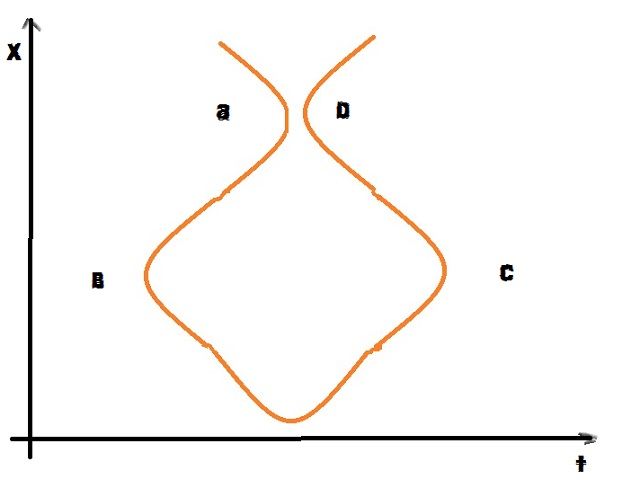
\includegraphics[scale=0.72]{Images/CC/P-Graphs/Common/Original/ClassicalApproach/signofacclnfromxt}%
\end{minipage}}
\begin{quote}
a) a

b) b

c) c

d) d 

\{ Hint: By the above mentioned propositions, d) is the required section
with positive velocity and negative accleration. \}
\end{quote}

\subsection{\index{The Average-Velocity / Instantaneous Velocity , Equal Case}The
Average-Velocity / Instantaneous Velocity , Equal Case}
\begin{quote}
We know , that ( in a x-t graph) the slope of the Secant is the Average
Velocity , whereas the slope of Tangent is the Instaneous Velocity.
The point where these two lines coincide, is the point where Average
Velocity is equal to Instantaneous Velocity.
\end{quote}
\begin{description}
\item [{Example:}] Position-time graph is shown which is a semicircle from
t = 2 to t = 8 s. Find time t at which the instantaneous velocity
is equal to average velocity over first t seconds,
\end{description}
\begin{quote}
\doublebox{\begin{minipage}[t]{0.7\columnwidth}%
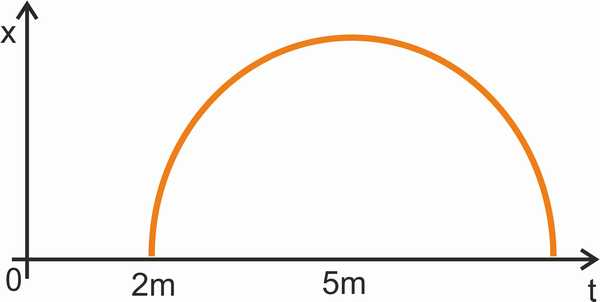
\includegraphics[scale=0.5]{Images/CC/P-Graphs/1e-1.1e/ImagesReduced/Q1-avinseq}%
\end{minipage}}

a) 4.8 s

b) 3.2 s

c) 2.4 s

d) 5 s

\{ Hint: The tangent from 0 to the circle is drawn. It's normal passes
through the center of the circle. Time at this instant needs to be
calculated.

If H=5 , R = 3 , Length of tangent = 4. (By Pythagoras.)

Angle which the tangent makes with the t axis is $\theta$ = $sin^{-1}(3/5)$

So, the projection of tangent on t axis ( i.e. the required time )
= 4 cos $\theta$ = $4\times\dfrac{4}{5}=3.2$

\doublebox{\begin{minipage}[t]{0.7\columnwidth}%
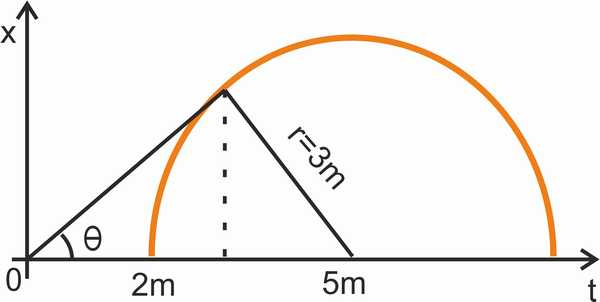
\includegraphics[scale=0.5]{Images/CC/P-Graphs/1e-1.1e/ImagesReduced/Q1-avinseq-Answer}%
\end{minipage}}

\}
\end{quote}

\subsection{\index{The Velocity-Displacement Case}The Velocity-Displacement
Case}
\begin{quote}
This can be handled in a similar way as Acceleration-Displacement
case by integrating the respective equation. Here the problem is of
v = f(x) type, which can be integrated by writing $\dfrac{dx}{dt}=f(x)$

i.e. dx = f(x)dt
\end{quote}
\begin{description}
\item [{Example:}] The velocity-displacement graph of a particle moving
along a straight line is shown here.
\item [{%
\doublebox{\begin{minipage}[t]{0.7\columnwidth}%
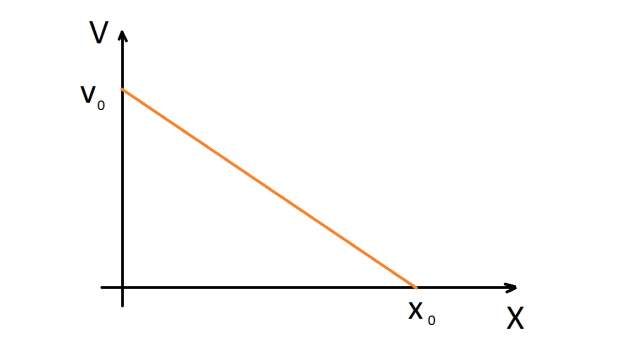
\includegraphics[scale=0.72]{Images/CC/P-Graphs/Common/Reduced/ClassicalApproach/velocitydisplacement}%
\end{minipage}}}]~
\end{description}
\begin{quote}
The most suitable acceleration-displacement graph will be

\doublebox{\begin{minipage}[t]{0.7\columnwidth}%
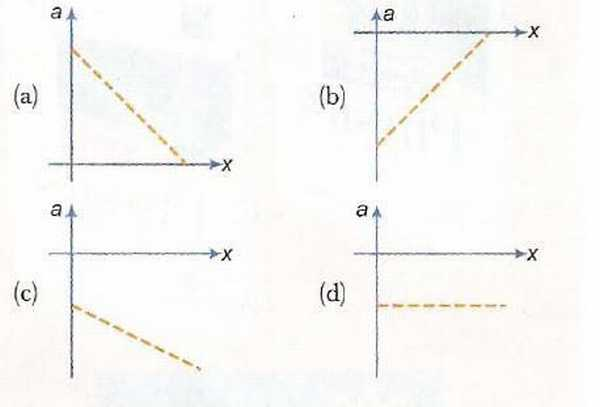
\includegraphics[scale=0.5]{Images/CC/P-Graphs/1e-1.1e/ImagesReduced/Q1-velocitydisplacementanswer}%
\end{minipage}}

\{Hint: Using Co-Ordinate Geometry Result studied in +1 Mathematics,
we get the equation of the graph

$\dfrac{v}{v_{o}}+\dfrac{x}{x_{o}}=1$

We are supposed to find the a-x graph from this.

So, we rewrite this equation as $v=v_{o}(1-\dfrac{x}{x_{o}})$

Differentiating, we get $a=-\dfrac{v_{o}}{x_{o}}=constant$

Hence d) is the requisite graph.

Answer: d) is the correct answer. \}
\end{quote}
\begin{description}
\item [{Example.}] The velocity (v) of a body moving along the postive
x-direction varies with displacement (x) from the origin as p v =
k x , where k is a constant. Which of the graphs shown in Fig. correctly
represents the displacement-time (x - t) graph of the motion?
\item [{%
\doublebox{\begin{minipage}[t]{0.7\columnwidth}%
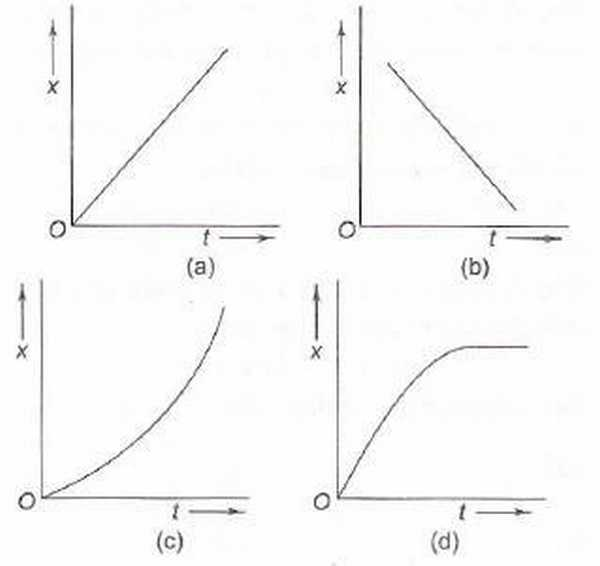
\includegraphics[scale=0.5]{Images/CC/P-Graphs/1e-1.1e/ImagesReduced/Q2-velocitydisplacement}%
\end{minipage}}}]~
\end{description}
\begin{quote}
\{Hint: The variable p removes the dependence of v on x and gives
emphasis only on the first condition that body is moving along positive
x-direction. In Graphs a) ,c) body is moving along positive x-direction,
However, a) is a specific case when p is proportional to x and not
the general case. Only c) covers the general case of all possible
p and still moving in positive x-direction. Hence c) is the correct
answer

Answer: c) is the required answer. \}
\end{quote}

\subsection{\index{Motion Under Free Fall}Motion Under Free Fall due to Gravity}
\begin{quote}
In such examples, the governing equations rule and the coordi-nate
system needs to be properly chosen.
\end{quote}
\begin{description}
\item [{Example:}] Which of the following graphs correctly represents velocity-time
relationship for a particle released from rest to fall freely under
gravity? 
\item [{%
\doublebox{\begin{minipage}[t]{0.7\columnwidth}%
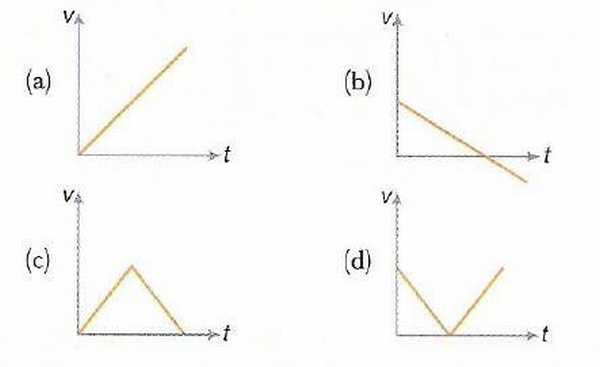
\includegraphics[scale=0.5]{Images/CC/P-Graphs/1e-1.1e/ImagesReduced/Q1-freefall}%
\end{minipage}}}]~
\end{description}
\begin{quote}
\{ Hint: If we take the downward axis as positive, v will keep on
increasing till the object hits something. 

So, a) is the correct answer.\}
\end{quote}
\begin{description}
\item [{Example:}] The velocity-time graph of a body falling from rest
under gravity and rebounding from a solid surface is represented by
which of the following graphs?
\item [{%
\doublebox{\begin{minipage}[t]{0.7\columnwidth}%
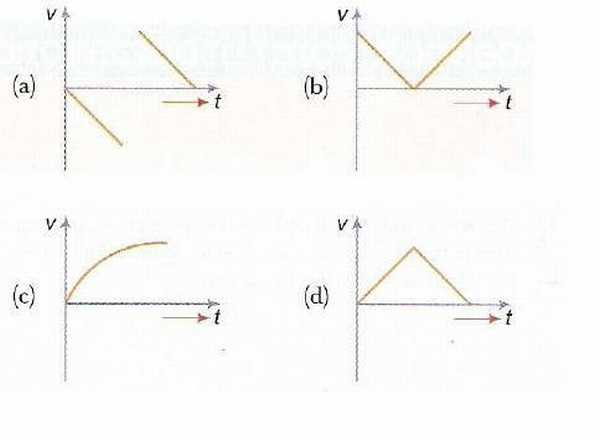
\includegraphics[scale=0.5]{Images/CC/P-Graphs/1e-1.1e/ImagesReduced/Q2-freefall}%
\end{minipage}}}]~
\end{description}
\begin{quote}
\{ Hint: At rebound, the velocity would become negative of itself
if the collision is perfectly elastic. Only in graph (a) such a thing
is happening. 

a) is the correct answer.\}
\end{quote}
\begin{description}
\item [{Example:}] A body A is thrown vertically upwards with such a velocity
that it reaches a maximum height of h. Simultaneously another body
B is dropped from height h. It strikes the ground and doesn't rebound.
The velocity of A relative to B vs time graph is best represented
by (upward direction is positive.)
\item [{%
\doublebox{\begin{minipage}[t]{0.7\columnwidth}%
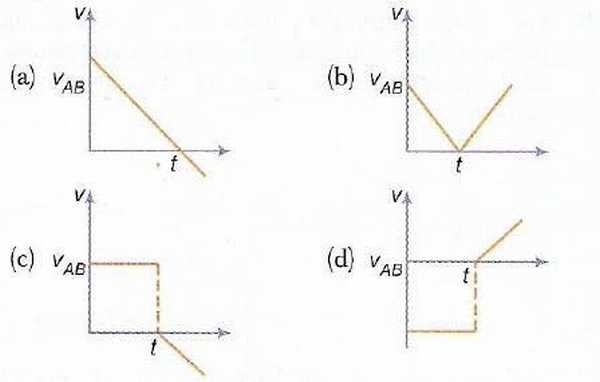
\includegraphics[scale=0.5]{Images/CC/P-Graphs/1e-1.1e/ImagesReduced/Q3-freefall}%
\end{minipage}}}]~
\end{description}
\begin{quote}
\{ Hint: Before the strike, body A has velocity u-gt whereas body
B has velocity -gt. So, a constant difference of u remains. Before
strike, u-gto+gto=u . However , after that it is u-gt , the time being
to=u/g of strike. So, the negative slope line starts from the x-axis
and a discontinuity comes into picture. 

So , C) is the required graph.\}
\end{quote}

\subsection{\index{Projectile Motion}Projectile Motion}
\begin{description}
\item [{Example:}] A shell is fired from a gun at an angle to the horizontal.
Graphs are drawn for its horizontal component of velocity $v_{x}$
and its vertical component of velocity $v_{y}$.
\item [{%
\doublebox{\begin{minipage}[t]{0.7\columnwidth}%
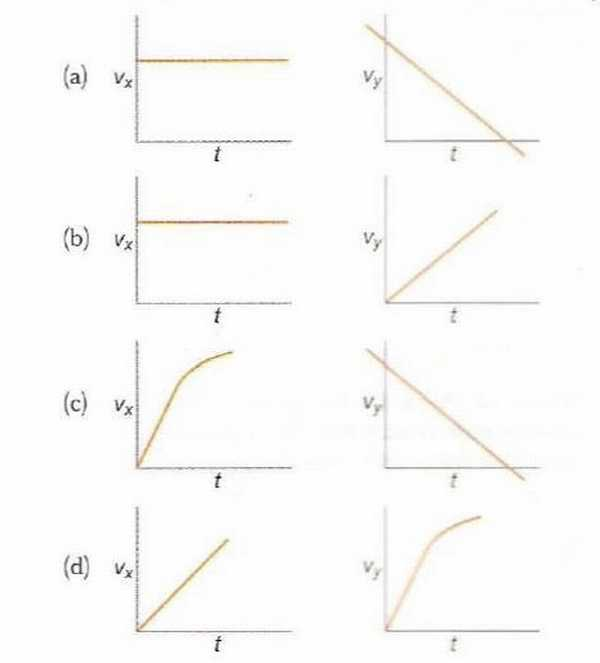
\includegraphics[scale=0.5]{Images/CC/P-Graphs/1e-1.1e/ImagesReduced/Q1-projectilemotion}%
\end{minipage}}}]~
\end{description}
\begin{quote}
\{ Hint: $v_{x}$ would remain constant as ucos$\theta$ and $v_{y}$
would linearly decrease and go negative after maximum height is attained(if
the fire angle is +ve).

So, a) is the requisite graph.\}
\end{quote}

\subsection{\index{Miscelleneous}Miscelleneous}
\begin{description}
\item [{Example.}] Figure shows the displacement-time ( x-t ) graph of
body moving in a straight line. Which one of the graphs shown in Fig.
represents the velocity- time ( v-t ) graph of the motion of the body.
\item [{%
\doublebox{\begin{minipage}[t]{0.7\columnwidth}%
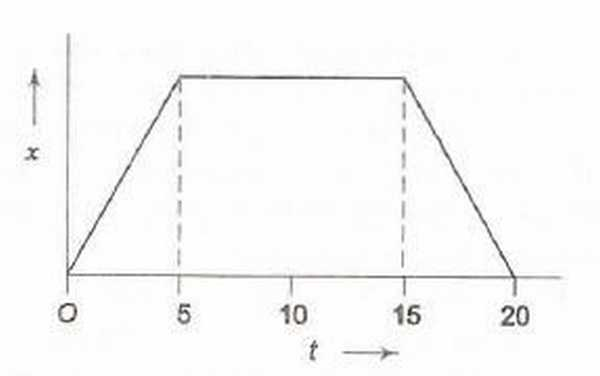
\includegraphics[scale=0.5]{Images/CC/P-Graphs/1e-1.1e/ImagesReduced/Q1-miscelleneous}%
\end{minipage}}}]~
\item [{%
\doublebox{\begin{minipage}[t]{0.7\columnwidth}%
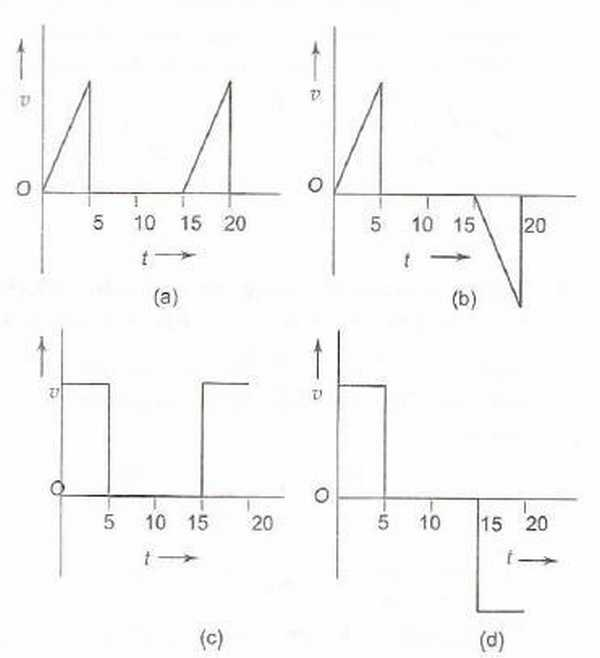
\includegraphics[scale=0.5]{Images/CC/P-Graphs/1e-1.1e/ImagesReduced/Q1-miscelleneous-Answers}%
\end{minipage}}}]~
\end{description}
\begin{quote}
\{ Hint: The graph has initially (0-5) a +ve slope, then zero slope
and then (15-20) an equal -ve slope

So, d) is the correct answer. \}
\end{quote}
\begin{description}
\item [{Example.}] Which of the displacement-time (x\textminus t) graphs
shown in Fig. can possibly represent one dimensional motion of a particle?
\item [{%
\doublebox{\begin{minipage}[t]{0.7\columnwidth}%
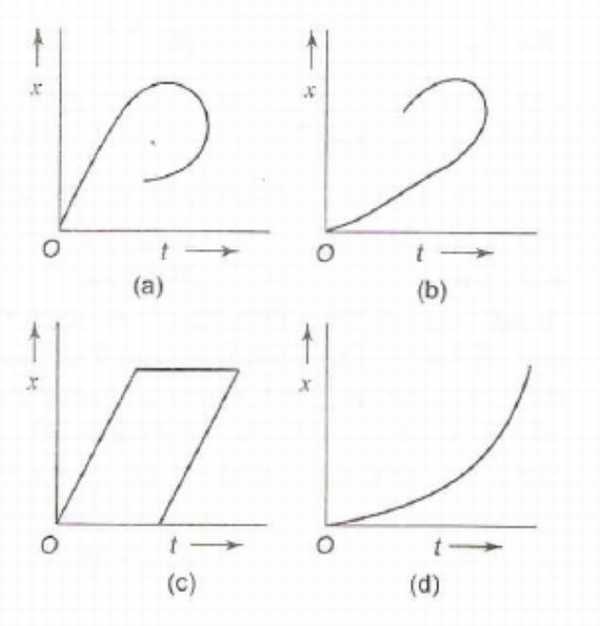
\includegraphics[scale=0.5]{Images/CC/P-Graphs/1e-1.1e/ImagesReduced/Q2-miscelleneous}%
\end{minipage}}}]~
\end{description}
\begin{quote}
\{ Hint: The object cannot be at two positions on a single time instant,

So, d) is the correct option. \}
\end{quote}
\begin{description}
\item [{Example.}] A car starts from rest, accelerates uniformly for 4
seconds and then moves with uniform velocity. Which of the (x-t) graphs
shown in Fig. represents the motion of the car upto t = 7 s?
\item [{%
\doublebox{\begin{minipage}[t]{0.7\columnwidth}%
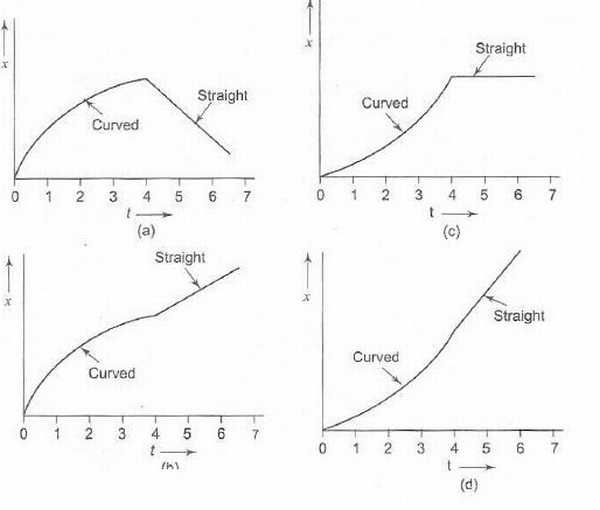
\includegraphics[scale=0.5]{Images/CC/P-Graphs/1e-1.1e/ImagesReduced/Q3-miscelleneous}%
\end{minipage}}}]~
\end{description}
\begin{quote}
\{ Hint: As the car is accelerating upto 4 seconds, the graph should
be concave up. Further ahead , it moves with constant velocity , so
a positive slope ahead of 4 seconds. 

d) is the correct answer. \}
\end{quote}
\begin{description}
\item [{Example.}] Two stones are thrown up simultaneously with initial
speeds of $u_{1}$ and $u_{2}$, ($u_{2}$ \textgreater{} $u_{1}$)
. They hit the ground after 6 s and 10 s respectively. Which graph
in Fig. correctly represents the time variation of $\triangle x=x_{2}-x_{1}$,
the relative position of the second stone with respect to the first
upto t = 10 s? Assume that the stones do not rebound after hitting
the ground.
\item [{%
\doublebox{\begin{minipage}[t]{0.7\columnwidth}%
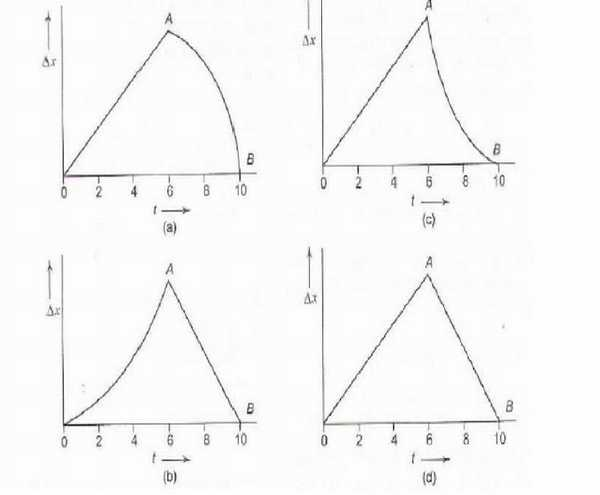
\includegraphics[scale=0.5]{Images/CC/P-Graphs/1e-1.1e/ImagesReduced/Q4-miscelleneous}%
\end{minipage}}}]~
\end{description}
\begin{quote}
\{ Hint : While both are in air, the differece of their velocity vectors
would be a constant vector , so $\triangle x=c_{1}t$ . Also, after
the first stone hits ground, $\triangle x=c_{2}t-x_{o}$ as the velocity
component in x direction of second stone is constant. There is no
discontinutiy. So, both before and after one hits the ground , it
would be a straight line. 

Hence, d) is the correct answer. \}
\end{quote}
\begin{description}
\item [{Example.}] Figure shows the velocity-time (v - t) graphs for one
dimensional motion. But only some of these can be realized in practice.
These are
\item [{%
\doublebox{\begin{minipage}[t]{0.7\columnwidth}%
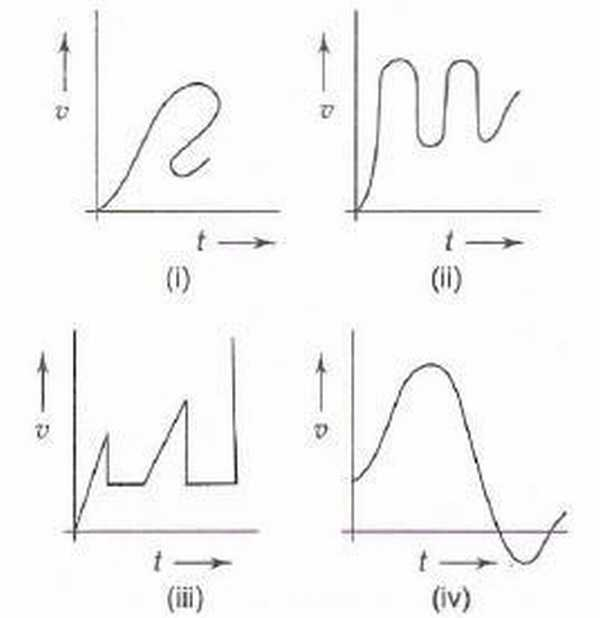
\includegraphics[scale=0.5]{Images/CC/P-Graphs/1e-1.1e/ImagesReduced/Q5-miscelleneous}%
\end{minipage}}}]~
\end{description}
\begin{quote}
a) (i), (ii) and (iv) only

b) (i), (ii) and (iii) only

c) (ii) and (iv) only

d) all

\{ Hint: At one particular instant, the object cannot have two different
velocities. 

Hence, c) is the correct answer. \}
\end{quote}
\begin{description}
\item [{Example.}] Which of the velocity-time (v-t) graphs shown in Fig.
can possibly represent one-dimensional motion of a particle?
\item [{%
\doublebox{\begin{minipage}[t]{0.7\columnwidth}%
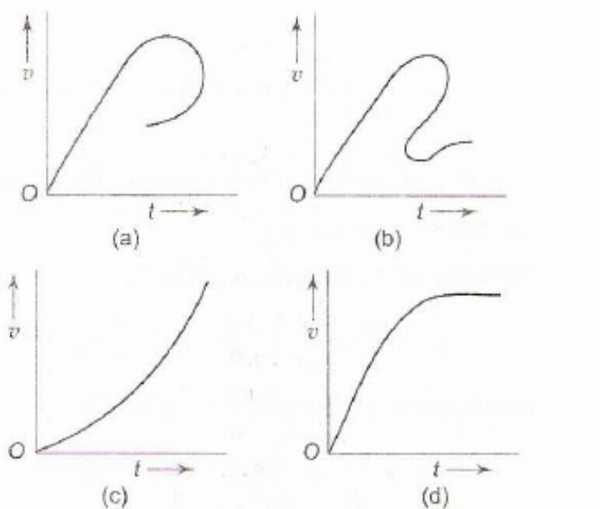
\includegraphics[scale=0.5]{Images/CC/P-Graphs/1e-1.1e/ImagesReduced/Q6-miscelleneous}%
\end{minipage}}}]~
\end{description}
\begin{quote}
\{Hint: In c) , the particle is constantly increasing in one dimension,
In d) , it stops near the end.

c),d) are the correct answers. \}
\end{quote}

\section{Question Types}

\subsection{Passage Type}
\begin{description}
\item [{Example:}] The speed-time graph of the motion of a body is shown
in Fig.
\item [{%
\doublebox{\begin{minipage}[t]{0.7\columnwidth}%
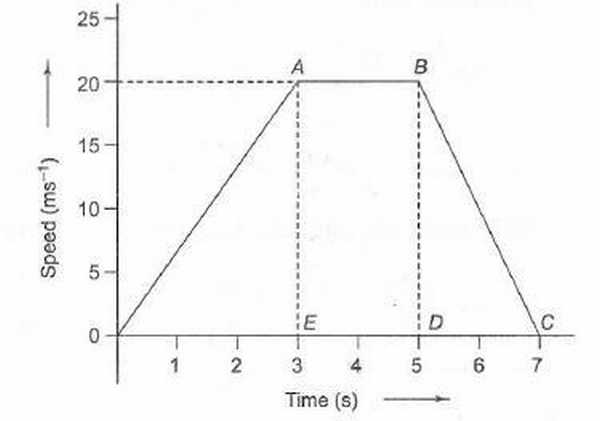
\includegraphics[scale=0.5]{Images/CC/P-Graphs/1e-1.1e/ImagesReduced/Q1-passagetype}%
\end{minipage}}}]~
\item [{1.}] The accelerations of the body during the last 2 second is 
\end{description}
\begin{quote}
a) $\dfrac{20}{3}ms^{-2}$

b) $-\dfrac{20}{7}ms^{-2}$

c) $-10ms^{-2}$

d) Zero
\end{quote}
\begin{description}
\item [{2.}] The ratio of distance travelled by the body during the last
2 seconds to the total distance travelled by it is 
\end{description}
\begin{quote}
a) 1/9 

b) 2/9 

c) 3/9 

d) 4/9
\end{quote}
\begin{description}
\item [{3.}] The average speed of the car during the whole journey is 
\end{description}
\begin{quote}
a) 10 m/s 

b) 20 m/s 

c) 90/7 m/s 

d) 40/7 m/s 

\{Hint: 1. As no contradictory statements are present, we would take
velocity as the value of speed only. Actually velocity is required
for calculation of acceleration but here , speed doesn't contradict
anything so we'll use it's value for velocity.

-10 from slope, c)

2. Speed time graph's area is distance. From area calculation, in
last 2 seconds, the area is 20 and total area is 90. 

So, 2/9 is the required ration b)

3. Total distance from area is 90, and total time is 7. 

So, 90/7. c)\}
\end{quote}
\begin{description}
\item [{Example:}] A body starts from rest at time t = 0 and undergoes
an acceleration as shown in Fig.Which of the graphs shown in Fig.
represents the velocity-time (v-t) graph of the motion of the body
from t = 0 s to t = 4 s? 
\item [{%
\doublebox{\begin{minipage}[t]{0.7\columnwidth}%
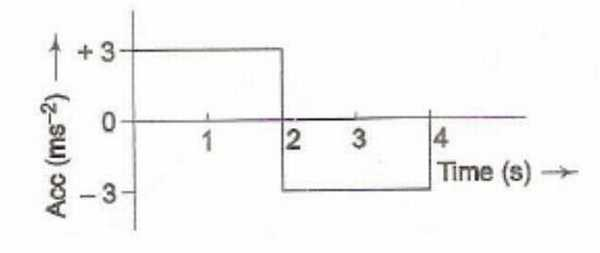
\includegraphics[scale=0.5]{Images/CC/P-Graphs/1e-1.1e/ImagesReduced/Q2-passagetype_im1}%
\end{minipage}}}]~
\item [{%
\doublebox{\begin{minipage}[t]{0.7\columnwidth}%
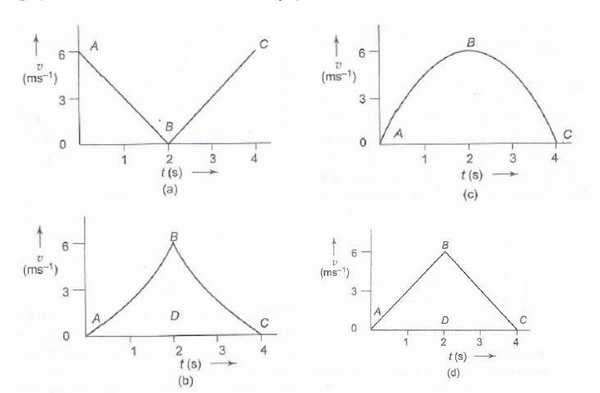
\includegraphics[scale=0.5]{Images/CC/P-Graphs/1e-1.1e/ImagesReduced/Q2-passagetype_im2}%
\end{minipage}}}]~
\end{description}
\begin{quote}
\{Hint: d) is the v-t graph by calculating area function.\}
\end{quote}
\begin{description}
\item [{1.}] In Question above, what is the velocity of the body at time
t = 2.5 s?
\end{description}
\begin{quote}
a) 2.5 m/s

b) 3.5 m/s

c) 4.5 m/s

d) 5.5 m/s
\end{quote}
\begin{description}
\item [{2.}] In above question, how much distance does the body cover from
t = 0 s to t = 4 s?
\end{description}
\begin{quote}
a) 6 m

b) 9 m

c) 12 m

d) 15 m
\end{quote}
\begin{description}
\item [{3}] In above question, which of the graphs shown in Fig. represents
the displacement-time (x-t) graph of the motion of the body from t
= 0 s to t = 4 s?
\item [{%
\doublebox{\begin{minipage}[t]{0.7\columnwidth}%
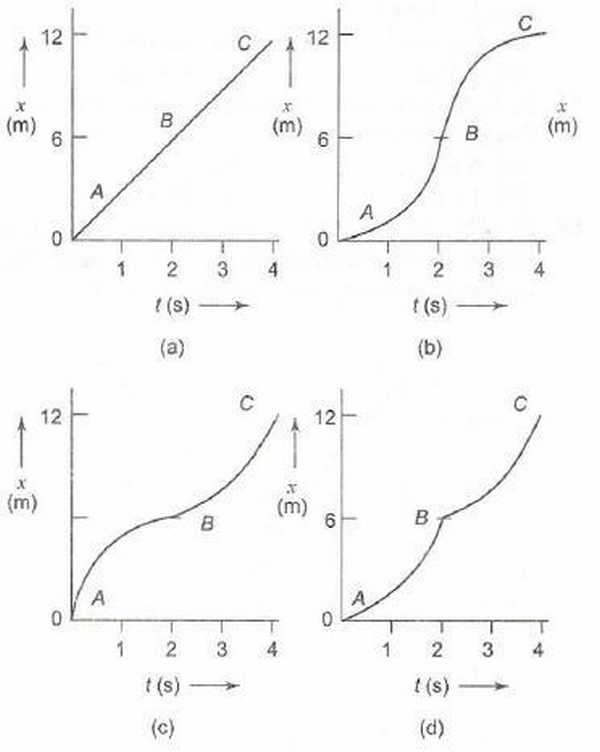
\includegraphics[scale=0.5]{Images/CC/P-Graphs/1e-1.1e/ImagesReduced/Q2-passagetype-Answers}%
\end{minipage}}}]~
\end{description}
\begin{quote}
\{ Hint: 1. The area under the accln-time graph gives change in velocity.
Till 2.5s, 6-1.5=4.5 is the required area. 

So, c)

2. Area under the v-t graph d) is 12 till 4 seconds. 

So, c)

3. Till 2 seconds , the graph should be concave-up while from 2 to
4 it should be concave-down.

So, b)

\}
\end{quote}

\subsection{Matching}
\begin{description}
\item [{1.}] Match the graphs (a), (b), (c) and (d) shown in Fig. with
the types of motions (p), (q), (r) and (s) that they represent
\item [{%
\doublebox{\begin{minipage}[t]{0.7\columnwidth}%
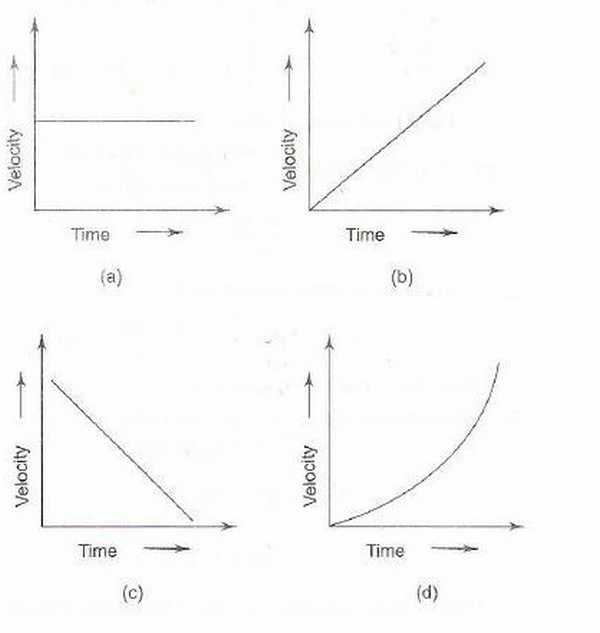
\includegraphics[scale=0.5]{Images/CC/P-Graphs/1e-1.1e/ImagesReduced/Q1-matchingtype}%
\end{minipage}}}]~
\end{description}
\begin{quote}
p) Motion with non-uniform acceleration

q) Motion of a body covering equal distances in equal intervals of
time

r) Motion having a constant retardation

s) Uniformly accelerated motion.

\{ Hint: p-\textgreater d , q-\textgreater a, r -\textgreater c
, s-\textgreater a,b,c \}
\end{quote}
\begin{description}
\item [{2.}] Figure shows the displacement �time (x - t) graph of the m-tion
of a body.
\item [{%
\doublebox{\begin{minipage}[t]{0.7\columnwidth}%
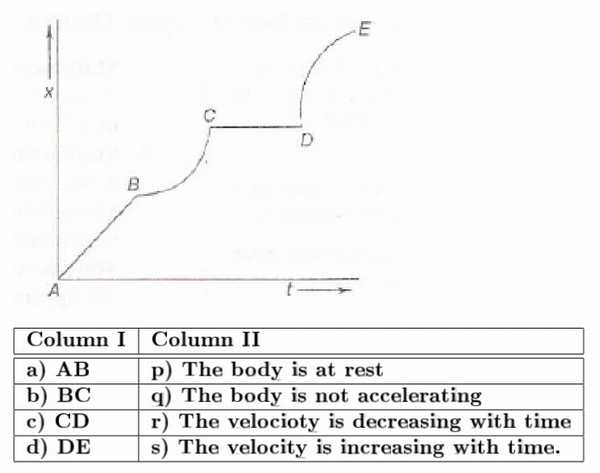
\includegraphics[scale=0.5]{Images/CC/P-Graphs/1e-1.1e/ImagesReduced/Q2-matchingtype}%
\end{minipage}}}]~
\item [{\{}] Hint p-\textgreater c, q-\textgreater a,c, r-\textgreater{}
d , s-\textgreater b \}
\end{description}

\section{\index{Previous Year Problems IIT}Previous Year Problems IIT}
\begin{description}
\item [{Q1:}] A particle starts from rest. Its acceleration ( a ) versus
time ( t ) is as shown in the gure. The maximum speed of the particle
will be
\item [{%
\doublebox{\begin{minipage}[t]{0.7\columnwidth}%
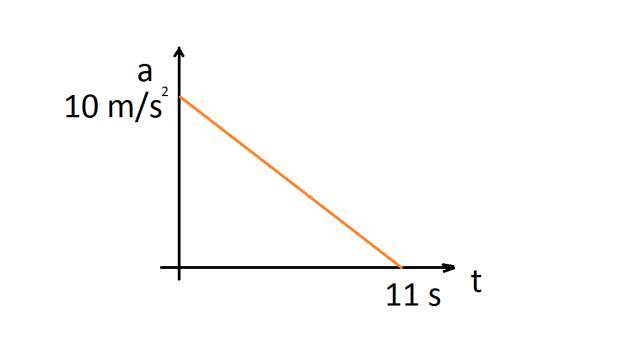
\includegraphics[scale=0.75]{Images/CC/P-Graphs/Common/Reduced/ClassicalApproach/accelerationvstime}%
\end{minipage}}}]~
\end{description}
\begin{quote}
a ) 110 m /s 

b ) 55 m /s 

c ) 550 m /s 

d ) 660 m /s

\{ Hint : See In chapter examples for solution. \}
\end{quote}
\begin{description}
\item [{Q2:}] If graph of velocity vs. distance is as shown, which of the
following graphs correctly represents the variation of acceleration
with displacement ?
\item [{%
\doublebox{\begin{minipage}[t]{0.7\columnwidth}%
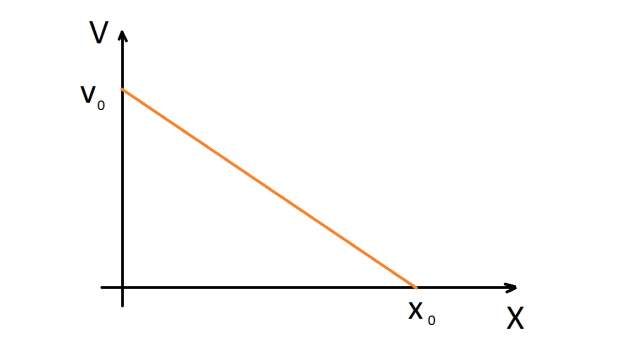
\includegraphics[scale=0.75]{Images/CC/P-Graphs/Common/Reduced/ClassicalApproach/velocitydisplacement}%
\end{minipage}}}]~
\item [{%
\doublebox{\begin{minipage}[t]{0.7\columnwidth}%
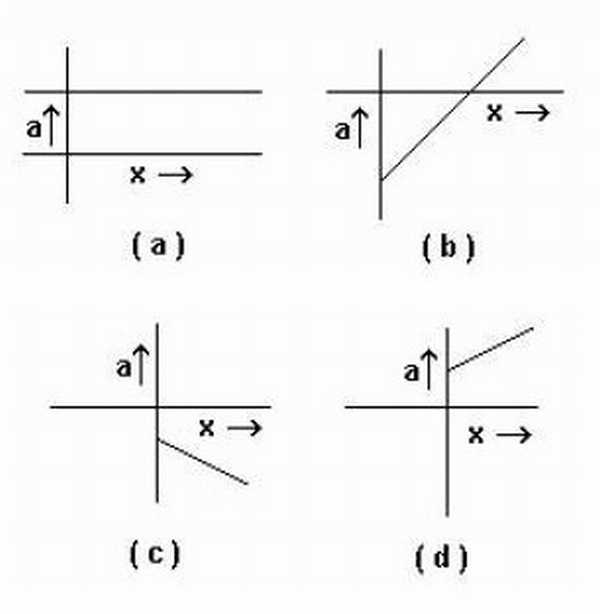
\includegraphics[scale=0.5]{Images/CC/P-Graphs/1e-1.1e/ImagesReduced/Q2-previousyearsiit_2}%
\end{minipage}}}]~
\end{description}
\begin{quote}
\{ Hint : The graph of the question is a straight line with the equation,
$\dfrac{x}{x_{o}}+\dfrac{v}{v_{o}}=1$ 

This gives , $v=v_{o}(1-x/x_{o})$

So, diffrentiating it, we get

$a=-v_{o}/x_{o}$ which is a constant. Only in a) it is shown to be
a constant. 

So, a) \}
\end{quote}
\begin{description}
\item [{Passage}] A lift is going up. The variation in the speed of the
lift is as given in the graph. 
\item [{%
\doublebox{\begin{minipage}[t]{0.7\columnwidth}%
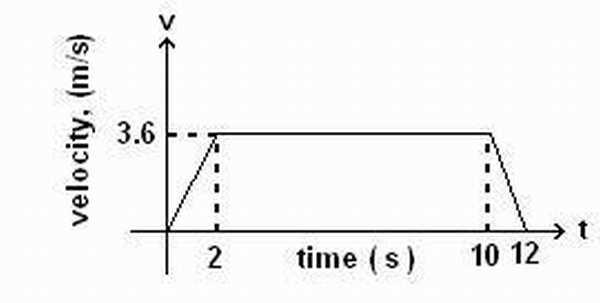
\includegraphics[scale=0.5]{Images/CC/P-Graphs/1e-1.1e/ImagesReduced/passage-previousyearsiit}%
\end{minipage}}}]~
\item [{Q3:}] What is the height to which the lift takes the passengers
? 
\end{description}
\begin{quote}
a ) 3.6 m 

b ) 28.8 m 

c ) 36 m

d ) cannot be calculated from the above graph
\end{quote}
\begin{description}
\item [{Q4:}] In the above graph, what is the average velocity of the lift? 
\end{description}
\begin{quote}
a ) 1 m/s 

b ) 2.88 m/s

c ) 3.24 m/s 

d ) 3 m/s 
\end{quote}
\begin{description}
\item [{Q5:}] In the above graph , what is the average acceleration of
the lift? 
\end{description}
\begin{quote}
a ) 1.8$m/s^{2}$ 

b ) \textminus 1.8$m/s^{2}$ 

c ) 0.3$m/s^{2}$ 

d ) zero 

\{Hint: Q3: Area under the graph is 36. Taking initial position as
zero, c) is the best fit answer.

Q4. For av. velocity, total displacement / total time should be calculated.
which is 36/12 = 3m/s . d ) is the required answer.

Q5. The accln is 1.8 from 0s to 2s, 0 from 2s to 10s and -1.8 from
10s to 12s. So, area under the a-t graph is zero. So av. accln is
zero d)

\}
\end{quote}
\begin{description}
\item [{Q6:}] Four persons K, L, M and N are initially at the corners of
a square of side of length d. If every person starts moving with velocity
v such that K is always headed towards L, L towards M, M towards N
and N towards K, then the four persons will meet after 
\end{description}
\begin{quote}
a ) d/v s 

b ) d2/ v s 

c ) d / 2v s 

d ) d / 2v s

\{Hint: Not a graphs question, we'll discuss it in kinematics book.
Athough an easy one. It was mistakenly added to graphs book. Let's
use it to signify the fact that even if a diagram is made, it is still
not a graph.\}
\end{quote}
\begin{description}
\item [{Example.}] A ball is dropped vertically from a height h above the
ground. It hits the ground and bounces up vertically to a height h/2.
Neglecting subsequent motion and air resistance, its velocity v varies
with the height h as (see Fig.) (l.l.T. 2000)
\item [{%
\doublebox{\begin{minipage}[t]{0.7\columnwidth}%
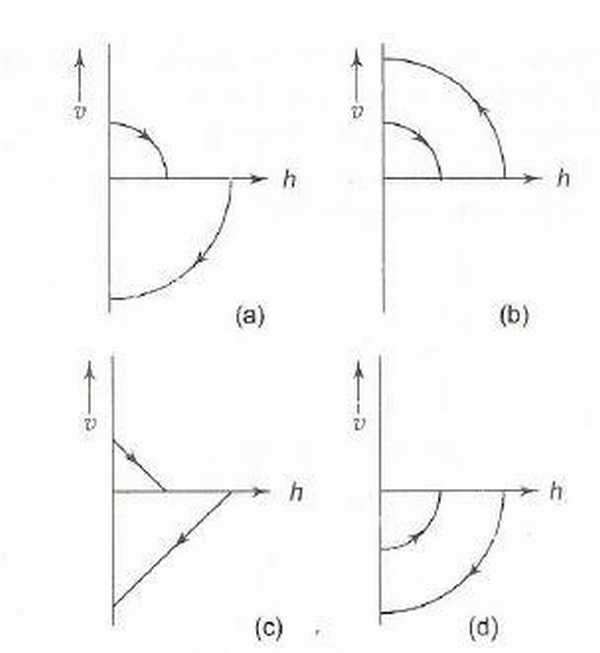
\includegraphics[scale=0.5]{Images/CC/P-Graphs/1e-1.1e/ImagesReduced/example-previousyearsiit}%
\end{minipage}}}]~
\end{description}
\begin{quote}
\{ Hint : Case 1: Thrown from height h with zero initial velocity,
v=-gt and h = $h_{o}-1/2gt^{2}$, so eliminating t, we get $h=h_{o}-v^{2}/2g$.
So, $v=-\sqrt{2g(h_{o}-h)}$

Case 2: We assume the opposite for solving purpose that the ball is
now thrown from a height $h_{o}/2$ and replace ho only and see the
effect. Taking upward velocity as positive , we get $v=\sqrt{2g(h_{o}/2-h)}$

a) is the required answer. \}

\printindex{}
\end{quote}

\end{document}
